\ifprintanswers
\begin{Envbox}
    \exerciselabel{Bonus \quad --- \quad Mots croisés version chimie \quad (\difficulty{3})}
    
    \begin{center}
        \centering
        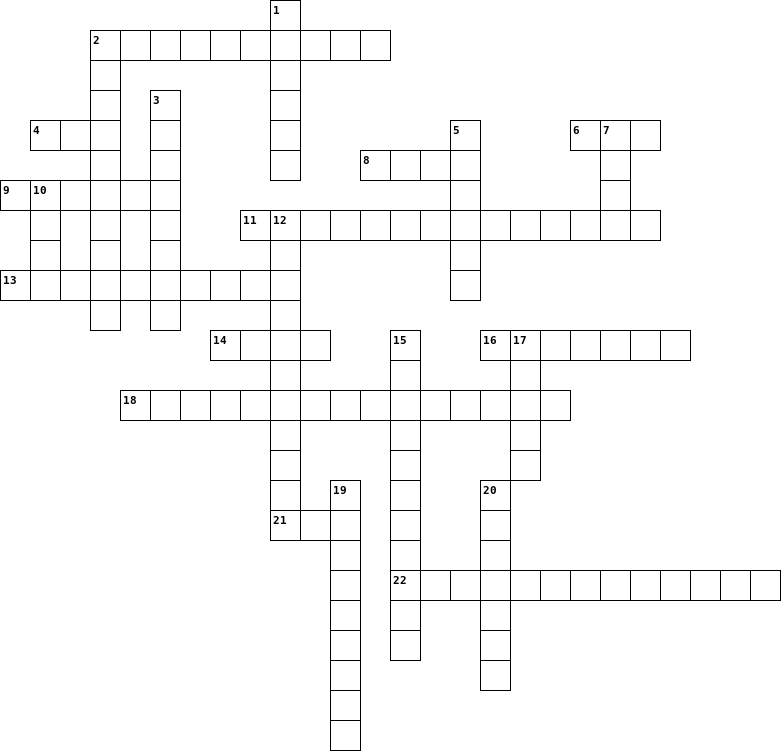
\includegraphics[width = \linewidth]{misc/mots-croises.png}
    \end{center}
    
    \renewcommand{\descriptionlabel}[1]{\textbf{\sffamily #1.}}
    \noindent\begin{minipage}{.45\linewidth}
    \noindent\paragraph{Horizontal}
    \begin{description}
		 \item[2] Il met la gomme
		 \item[4] C'est la base
		 \item[6] Blindée la base !
		 \item[8] Alcool aromatique
		 \item[9] Elles ont une odeur de pourri
		 \item[11] Promenade de doublets
		 \item[13] Divorce peu équitable
		 \item[14] Garde chiourme des ions métalliques
		 \item[16] Soude obèse
		 \item[18] Le cauchemar de M. Wurtz
		 \item[21] Standard quoique fictive
		 \item[22] Pour protéger les diols
    \end{description}
    \end{minipage}
    \begin{minipage}{.54\linewidth}
    \noindent\paragraph{Vertical}
    \begin{description}
		 \item[1] Ils ont une odeur de fruits
		 \item[2] Soude en déchéance
		 \item[3] Unité de cristallo
		 \item[5] Plus stable qu'une enveloppe
		 \item[7] On vous a déjà dit qu'il n'y a pas forcément de S$\textsc{n}$2 !
		 \item[10] Il y en a 12 dans 1g de carbone
		 \item[12] Parti en laissant derrière ses pensées négatives
		 \item[15] Attraction étrange
		 \item[17] D'une réputation sulfureuse
		 \item[19] Complexation carcérale
		 \item[20] A quelques neutrons près
    \end{description}
    \end{minipage}

\end{Envbox}
\fi